\documentclass[journal,12pt,twocolumn]{IEEEtran}
%
\usepackage{setspace}
\usepackage{gensymb}
\usepackage{xcolor}
\usepackage{caption}
%\usepackage{subcaption}
%\doublespacing
\singlespacing

%\usepackage{graphicx}
%\usepackage{amssymb}
%\usepackage{relsize}
\usepackage[cmex10]{amsmath}
\usepackage{mathtools}
%\usepackage{amsthm}
%\interdisplaylinepenalty=2500
%\savesymbol{iint}
%\usepackage{txfonts}
%\restoresymbol{TXF}{iint}
%\usepackage{wasysym}
\usepackage{hyperref}
\usepackage{amsthm}
\usepackage{mathrsfs}
\usepackage{txfonts}
\usepackage{stfloats}
\usepackage{cite}
\usepackage{cases}
\usepackage{subfig}
%\usepackage{xtab}
\usepackage{longtable}
\usepackage{multirow}
%\usepackage{algorithm}
%\usepackage{algpseudocode}
%\usepackage{enumerate}
\usepackage{enumitem}
\usepackage{mathtools}
%\usepackage{iithtlc}
%\usepackage[framemethod=tikz]{mdframed}
\usepackage{listings}


%\usepackage{stmaryrd}


%\usepackage{wasysym}
%\newcounter{MYtempeqncnt}
\DeclareMathOperator*{\Res}{Res}
%\renewcommand{\baselinestretch}{2}
\renewcommand\thesection{\arabic{section}}
\renewcommand\thesubsection{\thesection.\arabic{subsection}}
\renewcommand\thesubsubsection{\thesubsection.\arabic{subsubsection}}

\renewcommand\thesectiondis{\arabic{section}}
\renewcommand\thesubsectiondis{\thesectiondis.\arabic{subsection}}
\renewcommand\thesubsubsectiondis{\thesubsectiondis.\arabic{subsubsection}}

%\renewcommand{\labelenumi}{\textbf{\theenumi}}
%\renewcommand{\theenumi}{P.\arabic{enumi}}

% correct bad hyphenation here
\hyphenation{op-tical net-works semi-conduc-tor}

\lstset{
language=Python,
frame=single, 
breaklines=true,
columns=fullflexible
}



\begin{document}
%

\theoremstyle{definition}
\newtheorem{theorem}{Theorem}[section]
\newtheorem{problem}{Problem}
\newtheorem{proposition}{Proposition}[section]
\newtheorem{lemma}{Lemma}[section]
\newtheorem{corollary}[theorem]{Corollary}
\newtheorem{example}{Example}[section]
\newtheorem{definition}{Definition}[section]
%\newtheorem{algorithm}{Algorithm}[section]
%\newtheorem{cor}{Corollary}
\newcommand{\BEQA}{\begin{eqnarray}}
\newcommand{\EEQA}{\end{eqnarray}}
\newcommand{\define}{\stackrel{\triangle}{=}}
\bibliographystyle{IEEEtran}
%\bibliographystyle{ieeetr}
\providecommand{\nCr}[2]{\,^{#1}C_{#2}} % nCr
\providecommand{\nPr}[2]{\,^{#1}P_{#2}} % nPr
\providecommand{\mbf}{\mathbf}
\providecommand{\pr}[1]{\ensuremath{\Pr\left(#1\right)}}
\providecommand{\qfunc}[1]{\ensuremath{Q\left(#1\right)}}
\providecommand{\sbrak}[1]{\ensuremath{{}\left[#1\right]}}
\providecommand{\lsbrak}[1]{\ensuremath{{}\left[#1\right.}}
\providecommand{\rsbrak}[1]{\ensuremath{{}\left.#1\right]}}
\providecommand{\brak}[1]{\ensuremath{\left(#1\right)}}
\providecommand{\lbrak}[1]{\ensuremath{\left(#1\right.}}
\providecommand{\rbrak}[1]{\ensuremath{\left.#1\right)}}
\providecommand{\cbrak}[1]{\ensuremath{\left\{#1\right\}}}
\providecommand{\lcbrak}[1]{\ensuremath{\left\{#1\right.}}
\providecommand{\rcbrak}[1]{\ensuremath{\left.#1\right\}}}
\theoremstyle{remark}
\newtheorem{rem}{Remark}
\newcommand{\sgn}{\mathop{\mathrm{sgn}}}
\providecommand{\abs}[1]{\left\vert#1\right\vert}
\providecommand{\res}[1]{\Res\displaylimits_{#1}} 
\providecommand{\norm}[1]{\lVert#1\rVert}
\providecommand{\mtx}[1]{\mathbf{#1}}
\providecommand{\mean}[1]{E\left[ #1 \right]}
\providecommand{\fourier}{\overset{\mathcal{F}}{ \rightleftharpoons}}
\providecommand{\ztrans}{\overset{\mathcal{Z}}{ \rightleftharpoons}}
%\providecommand{\hilbert}{\overset{\mathcal{H}}{ \rightleftharpoons}}
\providecommand{\system}{\overset{\mathcal{H}}{ \longleftrightarrow}}
	%\newcommand{\solution}[2]{\textbf{Solution:}{#1}}
\newcommand{\solution}{\noindent \textbf{Solution: }}
\providecommand{\dec}[2]{\ensuremath{\overset{#1}{\underset{#2}{\gtrless}}}}
\numberwithin{equation}{section}
%\numberwithin{equation}{subsection}
%\numberwithin{problem}{subsection}
%\numberwithin{definition}{subsection}
\makeatletter
\@addtoreset{figure}{problem}
\makeatother
\let\StandardTheFigure\thefigure
%\renewcommand{\thefigure}{\theproblem.\arabic{figure}}
\renewcommand{\thefigure}{\theproblem}
%\numberwithin{figure}{subsection}
\def\putbox#1#2#3{\makebox[0in][l]{\makebox[#1][l]{}\raisebox{\baselineskip}[0in][0in]{\raisebox{#2}[0in][0in]{#3}}}}
     \def\rightbox#1{\makebox[0in][r]{#1}}
     \def\centbox#1{\makebox[0in]{#1}}
     \def\topbox#1{\raisebox{-\baselineskip}[0in][0in]{#1}}
     \def\midbox#1{\raisebox{-0.5\baselineskip}[0in][0in]{#1}}
\vspace{3cm}
\title{ 
%\logo{
Digital Signal Processing 
%}
%	\logo{Octave for Math Computing }
}
%\title{
%	\logo{Matrix Analysis through Octave}{\begin{center}\includegraphics[scale=.24]{tlc}\end{center}}{}{HAMDSP}
%}
% paper title
% can use linebreaks \\ within to get better formatting as desired
%\title{Matrix Analysis through Octave}
%
%
% author names and IEEE memberships
% note positions of commas and nonbreaking spaces ( ~ ) LaTeX will not break
% a structure at a ~ so this keeps an author's name from being broken across
% two lines.
% use \thanks{} to gain access to the first footnote area
% a separate \thanks must be used for each paragraph as LaTeX2e's \thanks
% was not built to handle multiple paragraphs
%
\author{ Rohith \\BM20BTECH11006 %<-this  stops a space
%\thanks{*The author is with the Department
%of Electrical Engineering, Indian Institute of Technology, Hyderabad
%502285 India e-mail:  gadepall@iith.ac.in.  All content in the manuscript is 
%released under GNU GPL.  Free to use for anything. }% <-this % stops a space
%\thanks{J. Doe and J. Doe are with Anonymous University.}% <-this % stops a space
%\thanks{Manuscript received April 19, 2005; revised January 11, 2007.}}
}
% note the % following the last \IEEEmembership and also \thanks - 
% these prevent an unwanted space from occurring between the last author name
% and the end of the author line. i.e., if you had this:
% 
% \author{....lastname \thanks{...} \thanks{...} }
%                     ^------------^------------^----Do not want these spaces!
%
% a space would be appended to the last name and could cause every name on that
% line to be shifted left slightly. This is one of those "LaTeX things". For
% instance, "\textbf{A} \textbf{B}" will typeset as "A B" not "AB". To get
% "AB" then you have to do: "\textbf{A}\textbf{B}"
% \thanks is no different in this regard, so shield the last } of each \thanks
% that ends a line with a % and do not let a space in before the next \thanks.
% Spaces after \IEEEmembership other than the last one are OK (and needed) as
% you are supposed to have spaces between the names. For what it is worth,
% this is a minor point as most people would not even notice if the said evil
% space somehow managed to creep in.
% The paper headers
%\markboth{Journal of \LaTeX\ Class Files,~Vol.~6, No.~1, January~2007}%
%{Shell \MakeLowercase{\textit{et al.}}: Bare Demo of IEEEtran.cls for Journals}
% The only time the second header will appear is for the odd numbered pages
% after the title page when using the twoside option.
% 
% *** Note that you probably will NOT want to include the author's ***
% *** name in the headers of peer review papers.                   ***
% You can use \ifCLASSOPTIONpeerreview for conditional compilation here if
% you desire.
% If you want to put a publisher's ID mark on the page you can do it like
% this:
%\IEEEpubid{0000--0000/00\$00.00~\copyright~2007 IEEE}
% Remember, if you use this you must call \IEEEpubidadjcol in the second
% column for its text to clear the IEEEpubid mark.
% make the title area
\maketitle
%\newpage
\tableofcontents
%\renewcommand{\thefigure}{\thesection.\theenumi}
%\renewcommand{\thetable}{\thesection.\theenumi}
\renewcommand{\thefigure}{\theenumi}
\renewcommand{\thetable}{\theenumi}
%\renewcommand{\theequation}{\thesection}
\bigskip
\begin{abstract}
This manual provides a simple introduction to digital signal processing.
\end{abstract}
\section{Software Installation}
Run the following commands
\begin{lstlisting}
sudo apt-get update
sudo apt-get install libffi-dev libsndfile1 python3-scipy  python3-numpy python3-matplotlib 
sudo pip install cffi pysoundfile 
\end{lstlisting}
\section{Digital Filter}
\begin{enumerate}[label=\thesection.\arabic*
,ref=\thesection.\theenumi]
\item
\label{prob:input}
Download the sound file from  
\begin{lstlisting}
wget https://github.com/Rohitkukutlla19/EE3900/blob/main/Assignment1/codes/Sound_Noise.wav
\end{lstlisting}
%\href{http://tlc.iith.ac.in/img/sound/Sound_Noise.wav}{\url{http://tlc.iith.ac.in/img/sound/Sound_Noise.wav}}  
%in the link given below.
%\linebreak
\item
\label{prob:spectrogram}
You will find a spectrogram at \href{https://academo.org/demos/spectrum-analyzer}{\url{https://academo.org/demos/spectrum-analyzer}}. 
%\end{problem}
%%
%
%%\onecolumn
%%\input{./figs/fir}
%\begin{problem}
Upload the sound file that you downloaded in Problem \ref{prob:input} in the spectrogram  and play.  Observe the spectrogram. What do you find?
\\
%
\solution There are a lot of yellow lines between 440 Hz to 5.1 KHz.  These represent the synthesizer key tones. Also, the key strokes
are audible along with background noise.
\begin{figure}[!ht]
	\begin{center}
	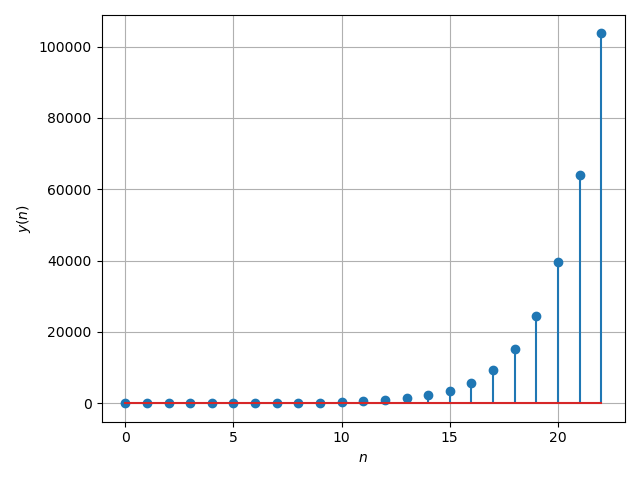
\includegraphics[width=\columnwidth]{./figs/2_2}
	\end{center}
	\captionof{figure}{}
	\label{fig:xnyn}	
	\end{figure}
% By observing spectrogram, it clearly shows that tonal frequency is under 4kHz. And above 4kHz only noise is present.
\item
\label{prob:output}
Write the python code for removal of out of band noise and execute the code.
\\
\solution
\begin{lstlisting}
import soundfile as sf
from scipy import signal
#read .wav file
input_signal,fs = sf.read('Sound_Noise.wav')
#sampling frequency of Input signal
sampl_freq=fs
#order of the filter
order=4
#cutoff frquency 4kHz
cutoff_freq=4000.0
#digital frequency
Wn=2*cutoff_freq/sampl_freq
# b and a are numerator and denominator polynomials respectively
b, a = signal.butter(order,Wn, 'low')
#filter the input signal with butterworth filter
output_signal = signal.filtfilt(b, a,input_signal)
#output signal = signal.lfilter(b, a,input signal)
#write the output signal into .wav file
sf.write('Sound With ReducedNoise.wav',output_signal, fs)
\end{lstlisting}
%\lstinputlisting{./codes/Cancel_noise.py}
%\begin{figure}[h]
%\centering
%\includegraphics[width=\columnwidth]{enc_block_diag.png}
%\caption{}
%\label{fig:convolution encoder}
%\end{figure}
%\input{block_enc}
\item
The output of the python script in Problem \ref{prob:output} is the audio file Sound\_With\_ReducedNoise.wav. Play the file in the spectrogram in Problem \ref{prob:spectrogram}. What do you observe?
\\
\solution The key strokes as well as background noise is subdued in the audio.  Also,  the signal is blank for frequencies above 5.1 kHz.
\begin{figure}[!ht]
	\begin{center}
	\includegraphics[width=\columnwidth]{./figs/2_4}
	\end{center}
	\captionof{figure}{}
	\label{fig:xnyn}	
	\end{figure}
\end{enumerate}
\section{Difference Equation}
\begin{enumerate}[label=\thesection.\arabic*,ref=\thesection.\theenumi]
\item Let
\begin{equation}
x(n) = \cbrak{\underset{\uparrow}{1},2,3,4,2,1}
\end{equation}
Sketch $x(n)$.
\item Let
\begin{multline}
\label{eq:iir_filter}
y(n) + \frac{1}{2}y(n-1) = x(n) + x(n-2), 
\\
 y(n) = 0, n < 0
\end{multline}
Sketch $y(n)$.  
\\
\solution The following code yields Fig. \ref{fig:xnyn}.
\begin{lstlisting}
wget https://github.com/Rohitkukutlla19/EE3900/blob/main/Assignment1/codes/3.2_xnyn.ipynb
\end{lstlisting}
\begin{figure}[!ht]
\begin{center}
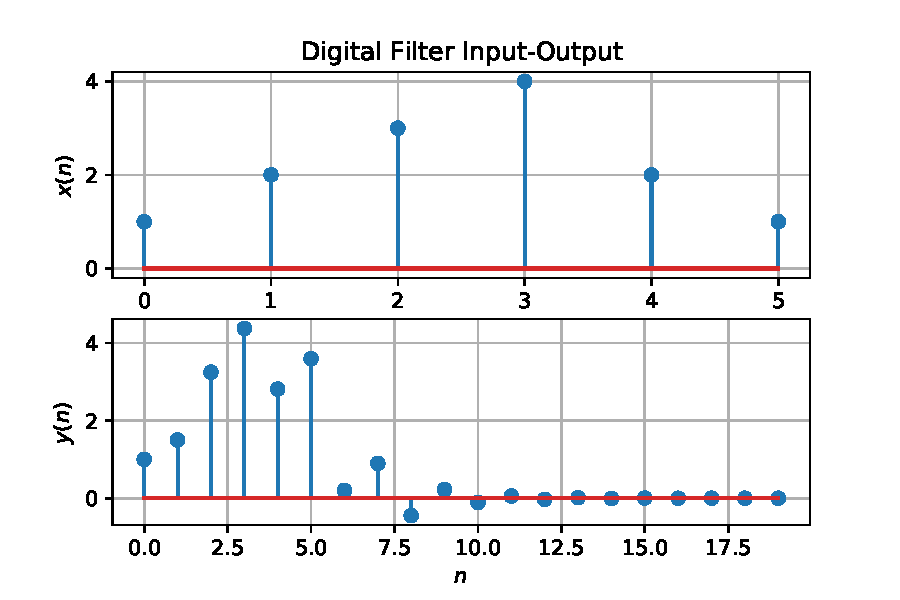
\includegraphics[width=\columnwidth]{./figs/xnyn}
\end{center}
\captionof{figure}{}
\label{fig:xnyn}	
\end{figure}
\item Repeat the above exercise using a C code.
\\
\solution The following code yields Fig. \ref{fig:xnyn}.
\begin{lstlisting}
wget https://github.com/Rohitkukutlla19/EE3900/blob/main/Assignment1/codes/3.3_xnyn.c
\end{lstlisting}
\begin{lstlisting}
#wget https://github.com/Rohitkukutlla19/EE3900/blob/main/Assignment1/codes/3.3_xnyn_1.ipynb
\end{lstlisting}
\begin{figure}[!ht]
\begin{center}

\includegraphics[width=\columnwidth]{./figs/xnyn_1}
\end{center}
\captionof{figure}{}
\label{fig:xnyn}	
\end{figure}
\end{enumerate}
\section{$Z$-transform}
\begin{enumerate}[label=\thesection.\arabic*]
\item The $Z$-transform of $x(n)$ is defined as
%
\begin{equation}
\label{eq:z_trans}
X(z)={\mathcal {Z}}\{x(n)\}=\sum _{n=-\infty }^{\infty }x(n)z^{-n}
\end{equation}
%
Show that
\begin{equation}
\label{eq:shift1}
{\mathcal {Z}}\{x(n-1)\} = z^{-1}X(z)
\end{equation}
and find
\begin{equation}
	{\mathcal {Z}}\{x(n-k)\} 
\end{equation}
\solution From \eqref{eq:z_trans},
\begin{align}
{\mathcal {Z}}\{x(n-k)\} &=\sum _{n=-\infty }^{\infty }x(n-1)z^{-n}
\\
&=\sum _{n=-\infty }^{\infty }x(n)z^{-n-1} = z^{-1}\sum _{n=-\infty }^{\infty }x(n)z^{-n}
\end{align}
resulting in \eqref{eq:shift1}. Similarly, it can be shown that
%
\begin{equation}
\label{eq:z_trans_shift}
	{\mathcal {Z}}\{x(n-k)\} = z^{-k}X(z)
\end{equation}
\item Obtain $X(z)$ for $x(n)$ defined in problem  $\eqref{X(n)}$.
\solution
\begin{align}
Z(x(n))&=\sum_{n=-\infty}^{\infty}x(n)z^{-n}\\
&=x(0)z^{0}+x(1)z^{-1}+x(2)z^{-2}+x(3)z^{-3}+\\
&\nonumber x(4)z^{-4}+x(5)z^{-5}\\
&=1+2z^{-1}+3z^{-2}+4z^{-3}+2z^{-4}+z^{-5}
\end{align}
\item Find
%
\begin{equation}
H(z) = \frac{Y(z)}{X(z)}
\end{equation}
%
from  \eqref{eq:iir_filter} assuming that the $Z$-transform is a linear operation.
\\
\solution  Applying \eqref{eq:z_trans_shift} in \eqref{eq:iir_filter},
\begin{align}
Y(z) + \frac{1}{2}z^{-1}Y(z) &= X(z)+z^{-2}X(z)
\\
\implies \frac{Y(z)}{X(z)} &= \frac{1 + z^{-2}}{1 + \frac{1}{2}z^{-1}}
\label{eq:freq_resp}
\end{align}
%
\item Find the Z transform of 
\begin{equation}
\delta(n)
=
\begin{cases}
1 & n = 0
\\
0 & \text{otherwise}
\end{cases}
\end{equation}
and show that the $Z$-transform of
\begin{equation}
\label{eq:unit_step}
u(n)
=
\begin{cases}
1 & n \ge 0
\\
0 & \text{otherwise}
\end{cases}
\end{equation}
is
\begin{equation}
U(z) = \frac{1}{1-z^{-1}}, \quad \abs{z} > 1
\end{equation}
\solution It is easy to show that
\begin{equation}
\delta(n) \ztrans 1
\end{equation}
and from \eqref{eq:unit_step},
\begin{align}
U(z) &= \sum _{n= 0}^{\infty}z^{-n}
\\
&=\frac{1}{1-z^{-1}}, \quad \abs{z} > 1
\end{align}
using the fomula for the sum of an infinite geometric progression.
%
\item Show that 
\begin{equation}
\label{eq:anun}
a^nu(n) \ztrans \frac{1}{1-az^{-1}} \quad \abs{z} > \abs{a}
\end{equation}
\solution
\begin{align}
{\mathcal {Z}}\{a^nu(n)\} &=\sum _{n=-\infty }^{\infty }a^nu(n)z^{-n}
\\
&=\sum _{n=-\infty }^{\infty }u(n) (az^{-1})^{n}
\\
&=\sum _{n=-\infty }^{\infty }(az^{-1})^{n} , \quad \abs{az^{-1}} < 1\\
\\
&= \frac{1}{1-az^{-1}} , \quad \abs{a} < \abs{z}
\end{align}
using the fomula for the sum of an infinite geometric progression.
%
\item 
Let
\begin{equation}
H\brak{e^{\j \omega}} = H\brak{z = e^{\j \omega}}.
\end{equation}
Plot $\abs{H\brak{e^{\j \omega}}}$.  Comment.  $H(e^{\j \omega})$ is
known as the {\em Discret Time Fourier Transform} (DTFT) of $x(n)$.
\\
\solution  The graph is symmetric and periodic it is attending high of value 4 and minimum between (0 - 0.5). 
It is bounded between (0, 4) and periodic with period $(2\pi)$
\\
\begin{align}
	H\brak{e^{j \omega}} &= \frac{1+e^{-2j\omega}}{1 + \frac{e^{-j\omega}}{2}}\\
	  \implies \abs{H\brak{e^{j \omega}}} &= \frac{\abs{1+e^{-2j\omega}}}{\abs{1 + \frac{e^{-j\omega}}{2}}}\\
						  &= \frac{\abs{1+e^{2j\omega}}}{\abs{e^{2j\omega} + \frac{e^{j\omega}}{2}}}\\
						  &= \frac{\abs{1+\cos2\omega + j\sin2\omega}}{\abs{e^{j\omega}+ \frac{1}{2}}}\\
						  &= \frac{\abs{4\cos^2\brak{\omega} + 4j\sin\brak{\omega}\cos\brak{\omega}}}{\abs{2e^{j\omega} + 1}}\\
						  &= \frac{\abs{4\cos\brak{\omega}}\abs{\cos\brak{\omega} + j\sin\brak{\omega}}}{\abs{2\cos\brak{\omega} + 1 + 2j\sin\brak{\omega}}}\\
	  \therefore \abs{H\brak{e^{j \omega}}} &= \frac{\abs{4\cos\brak{\omega}}}{\sqrt{5 +4\cos\brak{\omega}}}
  \end{align}
The following code plots Fig. \ref{fig:dtft}.
\begin{lstlisting}
wget https://github.com/yashrajput22/EE3900-22/blob/master/codes/Section-4/4_5.py
\end{lstlisting}
\begin{figure}[!ht]
\centering
\includegraphics[width=\columnwidth]{./figs/4_5}
\caption{$\abs{H\brak{e^{\j\omega}}}$}
\label{fig:dtft}
\end{figure}
\item Express $x(n)$ in terms of $H\brak{e^{\j \omega}}$.\\
\solution 
\begin{align}
	\int_{-\pi}^{\pi}e^{\j\omega(n - k)}d\omega =
	\begin{cases}
		2\pi & n = k \\
		0 & \textrm{otherwise}
	\end{cases}
\end{align}
\begin{align}
	H\brak{e^{j\omega}} &= \sum_{n=-\infty}^{\infty} h\brak{n} e^{-j\omega n}
	\\
	\int_{-\pi}^{\pi}H\brak{e^{j\omega}}e^{j\omega k}d\omega &= \sum_{n=-\infty}^{\infty} h\brak{n} \int_{-\pi}^{\pi} e^{-j\omega n}e^{j\omega k}d\omega
    \\
	\int_{-\pi}^{\pi}H\brak{e^{j\omega}}e^{j\omega k}d\omega &= \sum_{n=-\infty}^{\infty} h\brak{n} 2\pi
    \\
    \int_{-\pi}^{\pi}H\brak{e^{j\omega}}e^{j\omega k}d\omega &= 2\pi h\brak{n} 
	\\
	\frac{1}{2\pi} \int_{-\pi}^{\pi}H\brak{e^{j\omega}}e^{j\omega k}d\omega &= h\brak{n} 
\end{align} 
\end{enumerate}
\section{Impulse Response}
\begin{enumerate}[label=\thesection.\arabic*]
	\item Using long division, 
find
		\begin{align}
			h(n), \quad n < 5
		\end{align}
		for H(z) in 
		\eqref{eq:freq_resp}.
\item \label{prob:impulse_resp}
Find an expression for $h(n)$ using $H(z)$, given that 
%in Problem \ref{eq:ztransab} and \eqref{eq:anun}, given that
\begin{equation}
\label{eq:impulse_resp}
h(n) \ztrans H(z)
\end{equation}
and there is a one to one relationship between $h(n)$ and $H(z)$. $h(n)$ is known as the {\em impulse response} of the
system defined by \eqref{eq:iir_filter}.
\\
\solution From \eqref{eq:freq_resp},
\begin{align}
H(z) &= \frac{1}{1 + \frac{1}{2}z^{-1}} + \frac{ z^{-2}}{1 + \frac{1}{2}z^{-1}}
\\
\implies h(n) &= \brak{-\frac{1}{2}}^{n}u(n) + \brak{-\frac{1}{2}}^{n-2}u(n-2)
\end{align}
using \eqref{eq:anun} and \eqref{eq:z_trans_shift}.
\item Sketch $h(n)$. Is it bounded? Convergent? 
\\
\solution Yes, it is bounded between and convergent. We can clearly see in the plot it is not tending to infinite and remain finite.
\\
We see that $h(n)$ is bounded. For large $n$, we see that 
\begin{align}
	h(n) &= \brak{-\frac{1}{2}}^n + \brak{-\frac{1}{2}}^{n - 2} \\
		 &= \brak{-\frac{1}{2}}^{n}\brak{4 + 1} = 5\brak{-\frac{1}{2}}^n \\
		 &\implies \left|\frac{h(n + 1)}{h(n)}\right| = \frac{1}{2}
\end{align}
and therefore, $\lim_{n \to \infty}\left|\frac{h(n + 1)}{h(n)}\right| = \frac{1}{2} < 1$. Hence, we see that $h(n)$ converges.
\\
The following code plots Fig. \ref{fig:hn}.
\begin{lstlisting}
wget https://github.com/yashrajput22/EE3900-22/blob/master/codes/Section-5/5_2.py
\end{lstlisting}
\begin{figure}[!ht]
\centering
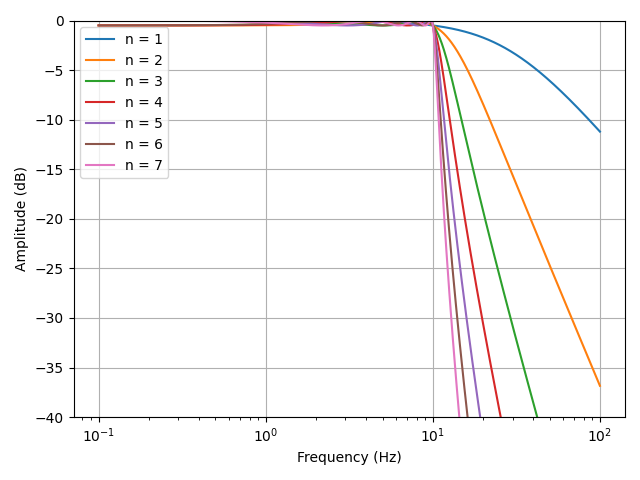
\includegraphics[width=\columnwidth]{./figs/5_2}
\caption{$h(n)$ as the inverse of $H(z)$}
\label{fig:hn}
\end{figure}
%
\item The system with $h(n)$ is defined to be stable if
\begin{equation}
\sum_{n=-\infty}^{\infty}h(n) < \infty
\end{equation}
Is the system defined by \eqref{eq:iir_filter} stable for the impulse response in \eqref{eq:impulse_resp}?
\\
\solution By using h(n) from 5.3
\begin{align}
h(n) &= \brak{-\frac{1}{2}}^{n}u(n) + \brak{-\frac{1}{2}}^{n-2}u(n-2)
\\
&= \sum_{n=-\infty}^{\infty} \brak{-\frac{1}{2}}^{n}u(n) + \brak{-\frac{1}{2}}^{n-2}u(n-2)
\\
&= \sum_{n=-\infty}^{\infty} \brak{-\frac{1}{2}}^{n}u(n) + \sum_{n=-\infty}^{\infty}  \brak{-\frac{1}{2}}^{n-2}u(n-2) 
\\
&= \sum_{n=-\infty}^{\infty} \brak{-\frac{1}{2}}^{n} + \sum_{n=-\infty}^{\infty}  \brak{-\frac{1}{2}}^{n-2}
\\
\\
&= \frac{2}{3} + \frac{2}{3} < \infty 
\end{align}
%
\item 
Compute and sketch $h(n)$ using 
\begin{equation}
\label{eq:iir_filter_h}
h(n) + \frac{1}{2}h(n-1) = \delta(n) + \delta(n-2), 
\end{equation}
%
This is the definition of $h(n)$.
\\
\solution The following code plots Fig. \ref{fig:hndef}. Note that this is the same as Fig. 
\ref{fig:hn}. 
\begin{align}
&= h(n) + \frac{1}{2}h(n-1) = \delta(n) + \delta(n-2)
\\
&= H(z) + \frac{1}{2}z^{-1}H(z) = 1+z^{-2}
\\
H(z) &= \frac{1}{1 + \frac{1}{2}z^{-1}} + \frac{ z^{-2}}{1 + \frac{1}{2}z^{-1}}
\\
h(n) &= \brak{-\frac{1}{2}}^{n}u(n) + \brak{-\frac{1}{2}}^{n-2}u(n-2)
\end{align}
%
\begin{lstlisting}
wget https://github.com/yashrajput22/EE3900-22/blob/master/codes/Section-5/5_4.py
\end{lstlisting}
\begin{figure}[!ht]
\centering
\includegraphics[width=\columnwidth]{./figs/5_4}
\caption{$h(n)$ from the definition}
\label{fig:hndef}
\end{figure}
%
\item Compute 
%
\begin{equation}
\label{eq:convolution}
y(n) = x(n)*h(n) = \sum_{n=-\infty}^{\infty}x(k)h(n-k)
\end{equation}
%
Comment. The operation in \eqref{eq:convolution} is known as
{\em convolution}.
%
\\
\solution The following code plots Fig. \ref{fig:ynconv}. Note that this is the same as 
$y(n)$ in  Fig. 
\ref{fig:xnyn}. 
%
\begin{lstlisting}
wget https://github.com/yashrajput22/EE3900-22/blob/master/codes/Section-5/5_5.py
\end{lstlisting}
We use Toeplitz matrices for convolution
\begin{align}
	\mtx{y} &= \mtx{x} \circledast \mtx{h}\\
	\mtx{y} &= 
	\begin{pmatrix}
		h_1 & 0 & . & . & . & 0 \\
		h_2 & h_1 & . & . & . & 0 \\
		h_3 & h_2 & h_1 & . & . & 0 \\
		. & . & . & . & . & . \\
		0 & . & . & h_3 & h_2 & h_1 \\
		0 & . & . & . & h_2 & h_1 \\
		0 & . & . & . & 0 & h_1
	\end{pmatrix}
	\begin{pmatrix}
		x_1 \\ x_2 \\ \vdots \\ x_n
	\end{pmatrix}
\end{align}
\begin{figure}[!ht]
\centering
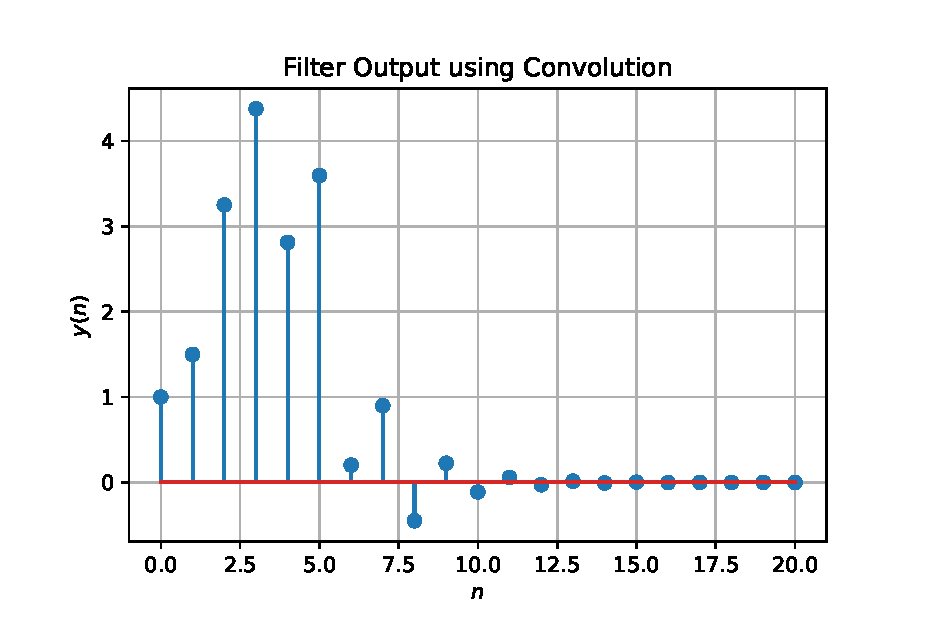
\includegraphics[width=\columnwidth]{./figs/ynconv}
\caption{$y(n)$ from the definition of convolution}
\label{fig:ynconv}
\end{figure}
\item Show that
\begin{equation}
y(n) =  \sum_{n=-\infty}^{\infty}x(n-k)h(k)
\end{equation}
\solution
From \eqref{eq:convolution}, we substitute $k := n - k$ to get
\begin{align}
y\brak{n} &= \sum_{k=-\infty}^{\infty}x\brak{k}h\brak{n - k} \\
		  &= \sum_{n - k=-\infty}^{\infty}x\brak{n - k}h\brak{k} \\
		  &= \sum_{k=-\infty}^{\infty}x\brak{n - k}h\brak{k}
\end{align}
\end{enumerate}
%
\section{DFT and FFT}
\begin{enumerate}[label=\thesection.\arabic*]
\item
Compute
\begin{equation}
X(k) \define \sum _{n=0}^{N-1}x(n) e^{-\j2\pi kn/N}, \quad k = 0,1,\dots, N-1
\end{equation}
and $H(k)$ using $h(n)$.
\item Compute 
\begin{equation}
Y(k) = X(k)H(k)
\end{equation}
\item Compute
\begin{equation}
 y\brak{n}={\frac {1}{N}}\sum _{k=0}^{N-1}Y\brak{k}\cdot e^{\j 2\pi kn/N},\quad n = 0,1,\dots, N-1
\end{equation}
\\
\solution The following code plots Fig. \ref{fig:ynconv}. Note that this is the same as 
$y(n)$ in  Fig. 
\ref{fig:xnyn}. 
%
\begin{lstlisting}
wget https://raw.githubusercontent.com/gadepall/EE1310/master/filter/codes/yndft.py
\end{lstlisting}
\begin{figure}[!ht]
\centering
\includegraphics[width=\columnwidth]{./figs/6_3}
\caption{$y(n)$ from the DFT}
\label{fig:yndft}
\end{figure}
\item Repeat the previous exercise by computing $X(k), H(k)$ and $y(n)$ through FFT and 
IFFT.
\item Wherever possible, express all the above equations as matrix equations.
\end{enumerate}
%
\section{Exercises}
Answer the following questions by looking at the python code in Problem \ref{prob:output}.
\begin{enumerate}[label=\thesection.\arabic*]
\item
The command
\begin{lstlisting}
	output_signal = signal.lfilter(b, a, input_signal)
	\end{lstlisting}
in Problem \ref{prob:output} is executed through the following difference equation
\begin{equation}
\label{eq:iir_filter_gen}
 \sum _{m=0}^{M}a\brak{m}y\brak{n-m}=\sum _{k=0}^{N}b\brak{k}x\brak{n-k}
\end{equation}
%
where the input signal is $x(n)$ and the output signal is $y(n)$ with initial values all 0. Replace
\textbf{signal.filtfilt} with your own routine and verify.
%
\item Repeat all the exercises in the previous sections for the above $a$ and $b$.
\item What is the sampling frequency of the input signal?
\\
\solution
Sampling frequency(fs)=44.1kHZ.
\item
What is type, order and  cutoff-frequency of the above butterworth filter
\\
\solution
The given butterworth filter is low pass with order=2 and cutoff-frequency=4kHz.
%
\item
Modifying the code with different input parameters and to get the best possible output.
%
\end{enumerate}
\end{document}
Footer
